\section{Projectorganisatie}

De projectorganisatie is opgebouwd zoals afgebeeld in onderdstaand figuur. De projectgroep is in opdracht van van het bedrijf Hazeu Orchids.
Het project wordt vanuit de Haagse hogeschool begeleid door dhr. Brilleman. Zijn rol bij
dit project is om de projectgroep te adviseren, als klankbord te fungeren en de resultaten
te beoordelen. De projectleider is het communicatiepunt voor zowel de opdrachtgever, de
projectbegeleider als de projectgroep. Deze functie wordt bekleed door Ka Chun Tsang.
Verder is er voor vergaderingen een vaste notulist aangesteld die de besproken onderwerpen
en besluiten op papier zal vastleggen. Deze functie wordt vervuld door Jesper Tjauw-A-Hing.
Naast de functies als projectleider en de notulist houden zij net als de projectleden Remt Bertz en Erwin Damman zich bezig met de projectactiviteiten.

\begin{figure}[h]
	\centering
	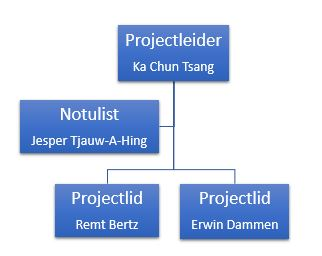
\includegraphics[width=\textwidth]{Afbeeldingen/Organisatie.JPG}
	\caption{Organisatie} 
\end{figure}

\newpage

\subsection{Projectleden}

\textbf{Projectleider}
ka Chun Tsang\\
Email: 09063684@student.hhs.nl\\[0.5cm]

textbf{Projectlid}
Remt Bertz\\
Email: 14092549@student.hhs.nl\\[0.5cm]

\textbf{Projectleider}
Erwin Dammen\\
Email: 14133917@student.hhs.nl\\[0.5cm]

\textbf{Projectleider}
Jesper Tjauw-A-Hing\\
Email: 14034697@student.hhs.nl\\[0.5cm]


\newpage